\documentclass[]{IEEEtran}
% some very useful LaTeX packages include:
%\usepackage{cite}      
\usepackage{graphicx}   
\usepackage{subfigure} 
\usepackage{url}       
\usepackage{amsmath}    
\usepackage{caption2}
% Your document starts here!
\begin{document}

% Define document title and author
	\title{Weekly Report}
	\author{Adviser: Prof. Yang Wen \\Student: Cheng Wensheng\\ Period: 2018.10.14-10.20
	}
	\markboth{Visual Information Processing Group}{}
	\maketitle

% Write abstract here
\begin{abstract}
	This week I mainly put my effort on going to Beijing to discuss project details and reading the paper about feature fusion semantic segmentation.
\end{abstract}

% Each section begins with a \section{title} command
\section{Paper reading}
	% \PARstart{}{} creates a tall first letter for this first paragraph
	\PARstart{T}{he} paper's title is \emph{ExFuse: Enhancing Feature Fusion for Semantic Segmentation}. In this paper, they propose a new framework, named ExFuse, to bridge the gap between low-level and high-level features thus significantly improve the segmentation quality by 4.0\% in total. In summary, following points show their main contributions:
	\begin{itemize}
		\item They suggest a new perspective to boost semantic segmentation performance, i.e. bridging the semantic and resolution gap between low-level and high-level features by more effective feature fusion.
		\item They propose a novel framework named ExFuse, which introduces more semantic information into low-level features and more spatial high-resolution
		information into high-level features. Significant improvements are obtained from the enhanced feature fusion.		
		\item They evaluate their approach on the challenging PASCAL VOC 2012 segmentation benchmark and achieve 87.9\% mean IoU, which outperforms the previous state-of-the-art results.
	\end{itemize}
	
	Fig.~\ref{fig:fw} is fusion methods of low-level and high-level features.
	

% Main Part

\newpage
\begin{figure}[!hbt]
%		 Center the figure.
		\vspace{0.5cm}
%		\hspace{50cm}
		\begin{center}
			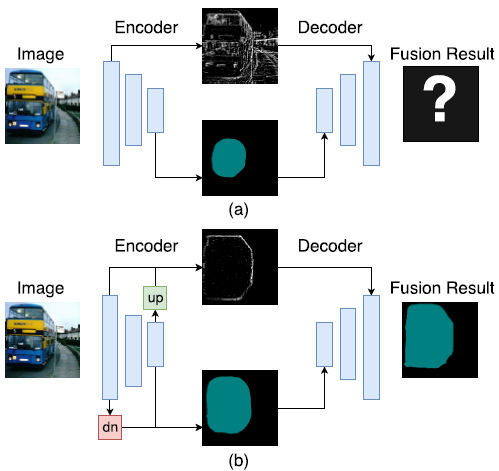
\includegraphics[width=\columnwidth]{fw}
				%		 Create a subtitle for the figure.
			\caption{Fusion methods of low-level and high-level features.}
			\label{fig:fw}

		\end{center}
	\end{figure}

% Your document ends here!
\end{document}